\documentclass[DIN, pagenumber=false, fontsize=11pt, parskip=half]{scrartcl}

\usepackage{amsmath}
\usepackage{amsfonts}
\usepackage{amssymb}
\usepackage{enumitem}
\usepackage[utf8]{inputenc} % this is needed for umlauts
\usepackage[ngerman]{babel} % this is needed for umlauts
\usepackage[T1]{fontenc} 
\usepackage{commath}
\usepackage{xcolor}
\usepackage{booktabs}
\usepackage{float}
\usepackage{tikz-timing}
\usepackage{tikz}
\usepackage{multirow}
\usepackage{colortbl}
\usepackage{xstring}
\usepackage{circuitikz}

\usetikzlibrary{calc,shapes.multipart,chains,arrows}

\title{Grundlagen der Rechnerarchitektur}
\author{Tim Luchterhand, Paul Nykiel (Abgabegruppe 117)}

\begin{document}
    \maketitle
    \section{}
    \begin{figure}[H]
        \centering
        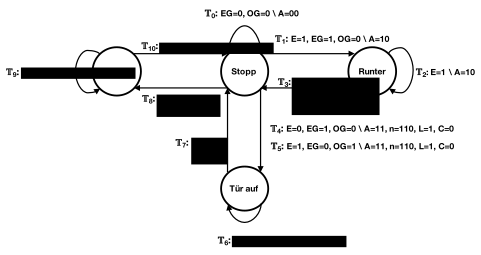
\includegraphics[width=\textwidth]{StateMachine.eps}
    \end{figure}

    \section{}
    \begin{figure}[H]
        \centering
        \includegraphics[width=\textwidth]{Transitionen.eps}
    \end{figure}
\end{document}

